\documentclass[a4paper,12pt]{article}
% Package to make citations superscrit with brackets
\usepackage[super,square]{natbib}
% Package to change margin size
\usepackage{anysize}
\marginsize{2cm}{2cm}{1cm}{2cm}
% Package to make headers
\usepackage{fancyhdr}
\renewcommand{\headrulewidth}{0pt}
% Package for highligths
\usepackage{soul}
% Colors for the references links
\usepackage[dvipsnames]{xcolor}
% Package to link references
\usepackage{hyperref}
\usepackage{animate}
\usepackage{graphicx}
\usepackage{float}
\hypersetup{
    colorlinks=true,
    linkcolor=black,
    citecolor=CadetBlue,
    filecolor=CadetBlue,      
    urlcolor=CadetBlue,
}
% Package for lorem ipsum
\usepackage{lipsum}
% Package for multicolumn
\usepackage{multicol}
\setlength\columnsep{18pt}
% Sets bastract
\renewenvironment{abstract}
 {\par\noindent\textbf{\abstractname} \ignorespaces:}
 {\par\noindent\medskip}

\begin{document}
\begin{center}
\Large{\textbf{Uke Tuner}}
\vspace{0.4cm}
\normalsize
\\ \textbf{Francesco Biancucci;} 984303 \\
\vspace{0.1cm}

\small{\textit{Laboratory of Making} 20/04/2023}
\medskip
\normalsize
\end{center}
{\color{gray}\hrule}
\vspace{0.4cm}
\begin{abstract}
The goal of the project was to design, program and build an automatic ukulele tuner which should be able to recognize the played note and then tune the selected string accordingly. The project was made of two main parts that needed to be designed and developed. The hardware, consisting of the circuit and the physical elements that made the motor interact with the uke and the software controlling the hardware.
\end{abstract}
{\color{gray}\hrule}
\medskip
\begin{multicols}{2}
\tableofcontents
\section{Introduction}
The project consists in a system designed to tune a ukulele without the user actively having to turn the keys. The initial idea was to create a somehow portable automatic uke tuner which uses a stepper motor to turn the uke keys in relation to the frequencies listened through a microphone. Everything needed to be controlled by an Arduino UNO R3, based on the Atmega328P chip. During the development of the project the idea shifted from a portable tuner to some sort of fixed station with four motors that needed only the uke to be put in it and then would tune the played string.\\
The final idea that was a compromise between the two because of two main reasons:
\begin{itemize}
    \item costs; using four motors makes the work easier and the project would look prettier, but the trade off between costs and the actual usefulness wasn't worth it.
    \item size; using a stepper motor such the one of choice doesn't actually save space, so the solution cannot be considered portable. Also the motor needs a decent amount of power to run, so the power supply adds to that.
\end{itemize}
\section{Hardware Design}
When talking about the system design we should consider two different components. The circuit part, with the selection of the different components that create the final design, and the software developed to actually control the hardware.
\subsection{Circuit}
The design of the circuit went through different iterations and changed in the time, following the changes that were made because of the knowledge acquired during the development process or the necessities that needed to be satisfied to make the system work.\\
The first version of the system used a L298N H-bridge, in Fig. \ref{fig:l298n}.
\begin{figure}[H]
        \begin{center}
            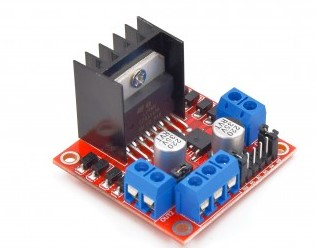
\includegraphics[width=5cm]{images/l298n.jpg}
            \caption{L298N}
            \label{fig:l298n}
        \end{center}
    \end{figure}
The L298N is a high voltage, high current dual full-bridge driver made of two integrated H-bridge inside that can support up to 46V and 2A per bridge. While with the L298N was possible to extract the source for powering the Arduino, it wasn't possible to control the output current that can go up to 2A. Such flow of current, if not handled, could damage the attached stepper motor. Moreover the dimensions of the L298N don't make it a versatile component that can be used in a circuit that doesn't take a lot of space.\\
For these reasons I decided to change from the L298N to the DRV8825 driver which allows for current flow control.
\begin{figure}[H]
    \begin{center}
        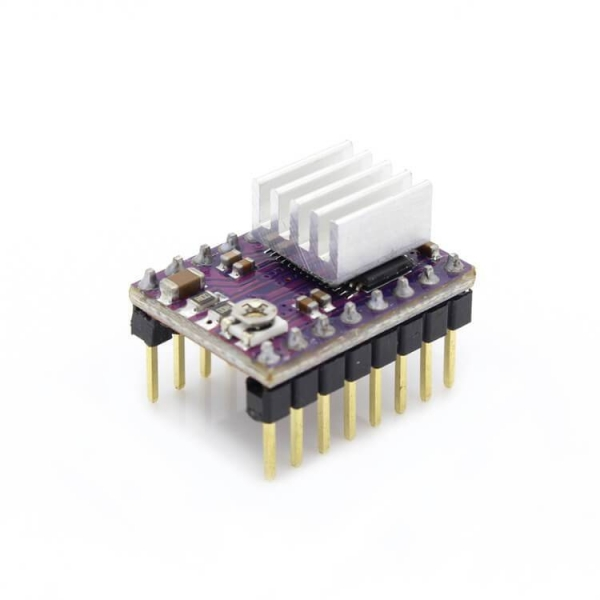
\includegraphics[width=5cm]{images/drv8825.jpg}
        \caption{DRV8825}
        \label{fig:drv8825}
    \end{center}
\end{figure}
\begin{figure}[H]
    \begin{center}
        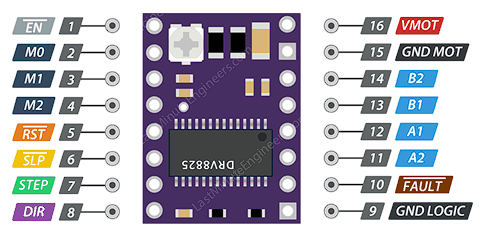
\includegraphics[width=7cm]{images/drv8825pinout.png}
        \caption{DRV8825 pinout}
        \label{fig:drv8825_pinout}
    \end{center}
\end{figure}
On a first glance it may seem an overkill but it has other useful functions that were then used inside the project. The first difference with the L298N, as said, is the ability to control the output current through an integrated resistor. The current limit is in fact determined by measuring the voltage at the ref pin (that is the resistor screw); the \textit{Vref} value should be half of the nominal current limit of the stepper.\\
By using Fig. \ref{fig:drv8825_pinout} I'll now explain the different meaning of the pins and what are the other functionalities offered by this driver.
\begin{itemize}
    \item EN is the enable pin and it is pulled LOW by default. When pulled LOW the driver is enabled, so by default the driver is enabled and can be used for a shutdown mechanism.
    \item MO, M1 and M2 are the pins used to define the step size resolution. By setting these pins to LOW/HIGH in combination is possible to control how much the stepper turns. By default these three pins are all pulled low meaning, as shown in Table \ref{tab:steps}, that the resolution is by defaul at full step. The final configuration of the driver actually used the half step to allow for better precision when turning the key.
    \item SLP is an active low pin that puts the driver to sleep when pulled LOW. It wasn't used since the tuner needs to be working almost all the time when it is powered on.
    \item RST is an active low pin too. When pulled Low the steps are ignored and it resets the driver.
    \item STEP is the controller of the microstpes of the motor. For each time it receives an HIGH pulse it drives the motor following the resolution of the microstep. E.g. if the stepper has a step of 1.8° and the resolution is full step then the motor rotates of 1.8°.
    \item DIR is the input pin that controls the direction of the motor. When pulled HIGH it turns the motor clockwise, counterclockwise when pulled LOW.
    \item VMOT e GNDMOT supply power to the motor. These pins can support a voltage between 8.2V and 45V. The module is not completely protected against voltage spikes, so as an additional protection a 100$\mu$F capacitor is put between the power supply and the pins.
    \item GND LOGIC is the ground for the logic level of the driver. It doesn't have an input logic pin since it has an internal 3V3 voltage regulator that allows the driver to drain from the motor power supply, but it needs the ground to be connected to the logic element.
    \item B2, B1, A1, A2 are the pins controlling the coils of the steppers.
    \item FAULT is a pin that when driven LOW disables the entire chip until reset or VMOT is removed. It is usually shorted to SLP.
\end{itemize}
The DRV8825 also comes with a small heatsink that helps in dissipating the heat.\\
The other elements that were changed during the development phase were the stepper itself, and I'll talk about it later, and the microphone. The first microphone used was suitable to detect audio but it wasn't able to detect the different frequencies, having only a digital output (i had this microphone already from another project). Then I switched to a microphone able to output a analog signal that could be interpreted. The problem this time around was that every sound was picked up so I ended going for the KY-037 microphone that has a reasonable precision on the analog readings and it also has a potentiometer on board that allows to adjust the threshold sensitivity.\\
\begin{figure}[H]
    \begin{center}
        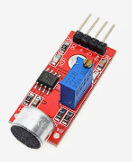
\includegraphics[width=3cm]{images/ky-037.PNG}
        \caption{ky-037}
        \label{fig:ky-037}
    \end{center}
\end{figure}
The other bits of circuitry used were two LEDs, one red and one green, used to signal if the uke string was in tune (green blink) or not (red blink). These two LEDs are connected on the 5V output line. Both LEDs have their own voltage drop and their rated current limit, from which the value of the resistances are computed. By using the Ohm's law \[V=R*I\] it is possible to get the resistances for the two LEDs.
\begin{itemize}
    \item Red led: 1.8V drop and 20mA rated current $\rightarrow$ R = (5-1.8)/0.02 = 160Ohm
    \item Green led: 2.0V drop and 20mA rated current $\rightarrow$ R = (5-2)/0.02 = 150Ohm
\end{itemize}
So i used two 200Ohm resistances.\\
The circuit also includes a LCD screen with a IIC adapter. The LCD is used to display some information during the tuning process, such as the selected string to tune or the played note when tuning. The LCD pins were soldered to the IIC adapter that allows for a smooth communication with the MCU and it also has a potentiometer on board that is used to regulate the back light of the LCD.
\begin{figure}[H]
    \begin{center}
        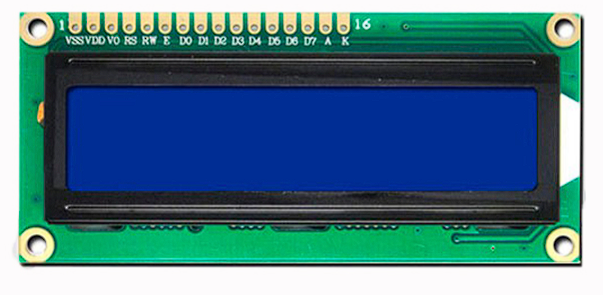
\includegraphics[width=5cm]{images/lcd1602.PNG}
        \caption{LCD}
        \label{fig:LCD}
    \end{center}
\end{figure}
To complete the circuit there is a switch that is used turn the LCD back light on and off.\\
It is reasonable to call the set of LCD and LEDs the control block of the tuner, since it is the part that allows to check the state of the tuning process. On this control block there are two more buttons and a potentiometer.\\
The first button is used to select the string to tune. After some considerations and after having studied other system used to tune guitars/ukuleles it was clear that the automatic process of recognizing the string that needs to be tuned is something that is based only on the "nearest string to the played tune" way of recognizing the string. For example if i played the G string, but the frequencies played were nearer to the A frequencies the tuner would default to tune to A. Since the system uses a motor to tune the string it was considered safer to select the string manually to avoid snapping the strings in case of a bad recognition happening.\\
The other button is used to manually turn the stepper to position the connector between the stepper and the uke key in a way that allows for connection. The potentiometer in this case is used to control the rotational speed of the motor.
\subsection{Stepper Motors}
The first used stepper motor in the project is the NEMA 17HS10-0704S that is a bipolar stepper motor with a step resolution of 1.8° and a rated current of 0.7A (Fig. \ref{fig:NEMA17HS10}. Following what has been said above the \textit{Vref} was set to 0.35A.
\begin{figure}[H]
    \begin{center}
        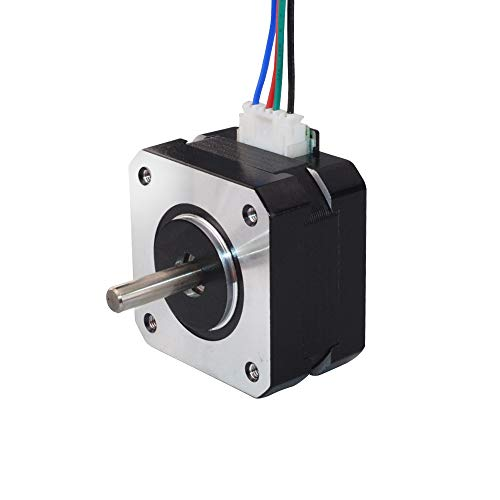
\includegraphics[width=5cm]{images/nema17-10.jpg}
        \caption{NEMA17-10}
        \label{fig:NEMA17-10}
    \end{center}
\end{figure}
As shown in the above figure the stepper has a cylindrical crankshaft that needs to be somehow connected to the uke key. There are couplers for this kind of crankshaft that can be bought but i also needed a way to connect the other end of the coupler to the key, so i decided to design my own coupler and my own connector. In Fig. \ref{fig:coupler} the coupler design si shown; to have a more accurate view it is possible to check the \href{https://github.com/Prop4et/LoM_Uketuner/blob/master/3D/coupler_part.stl}{stl file} loaded on github. The coupler has four sockets for the screws and for the nuts that are used to tighten it to the crankshaft. Since I designed the coupler I decided to create a little slot on the top of the crankshaft section that would help in keeping in place the fork used to lock the uke key (Fig. \ref{fig:grab}).
\begin{figure}[H]
    \centering
    \animategraphics[autoplay, loop, width=6cm]{24}{images/coupler/goupler-}{0}{167}
    \caption{Coupler}
    \label{fig:coupler}
\end{figure}
\begin{figure}[H]
    \centering
    \animategraphics[autoplay, loop, width=6cm]{24}{images/grab/grab-}{0}{82}
    \caption{Fork}
    \label{fig:grab}
\end{figure}
This design had some problems and needed to go different tries before being used. The first problem was that the measures used to design all the sockets were too precise and didn't take into account the tolerances that a 3D printer has. After a couple of iterations I managed to obtain a product that was usable, but during the test phase with the motor it showed two major issues:
\begin{itemize}
    \item The shape of the fork wasn't able to hold the key in place correctly, letting the key sliding laterally and then out of the fork
    \item The motor wasn't strong enought to turn the keys (I had adjusted the fork with a string on the outside that helped in keeping the key in place momentarily)
\end{itemize}
To solve the insufficient torque of the stepper I checked the pull out torque of the NEMA 17HS10 in Fig \ref{fig:NEMA17HS10torque} and then i tried the stepper with the settings at which the torque should be at its maximum point but it still didn't manage to turn the keys. So i changed the stepper and I went for a NEMA 17HS19 (in figure \ref{fig:nema17-19}) that has more torque and it also manages to keep almost the same amount of torque for a wider range of round per minutes (Fig. \ref{fig:NEMA17HS19torque}). This gives more room to work with and more room for error.
\begin{figure}[H]
    \begin{center}
        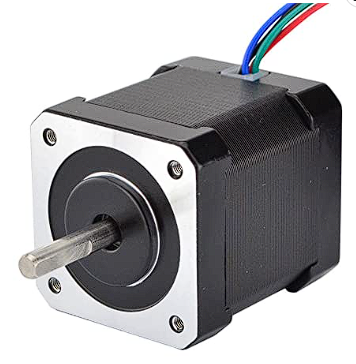
\includegraphics[width=5cm]{images/nema17-19.PNG}
        \caption{NEMA17-19}
        \label{fig:nema17-19}
    \end{center}
\end{figure}
The NEMA 17HS19 has a different crankshaft design too. There is a slice on the cylinder that made me rethink the design of the coupler not only on the fork side.
\begin{figure}[H]
    \centering
    \animategraphics[autoplay, loop, width=6cm]{24}{images/grabnew/grabnew-}{0}{97}
    \caption{Final coupler design}
    \label{fig:grabnew}
\end{figure}
For a better view of the new coupler design it could be helpful to check the \href{https://github.com/Prop4et/LoM_Uketuner/blob/master/3D/grabnew.stl}{.stl file}, but the main characteristics of this new coupler are:
\begin{itemize}
    \item built all in one piece, allowing for more precision since there is no tolerance in the movement of the fork with respect to the crankshaft 
    \item no screws needed, the small slice in the crankshaft allows for locking without needing to tighten the coupler, if the hole is of the right size
    \item the fork has four cylinders in a rectangular shape to lock the keys instead of three
\end{itemize}
Ideally this coupler works perfectly, but there are cases that even with the sliced section it slips, so i thought about adding two screholes on a side and removing a bit of material from a section of the cylinder, leaving an open space that will close up when tightening the screws. I don't know about the bending characteristics of the PLA though, so i opted for not trying that solution.\\
Another problem that showed with the coupler finally working is that che cylinders aren't fused strongly enouhg on the circular plate, so the strength needed to turn the keys sometimes caused a cylinder to snap.\\
The other two designed pieces create a system to keep the stepper in place and to align it to the keys of the uke. In fact the two forward keys are at a lower height than the back ones. So i created a holder (Fig. \ref{fig:holder}) for the stepper and a platform \ref{fig:platform} in wich the holder would slot in to make up for this height difference.
\begin{figure}[H]
    \centering
    \animategraphics[autoplay, loop, width=6cm]{24}{images/top/top-}{0}{91}
    \caption{Stepper holder}
    \label{fig:holder}
\end{figure}\begin{figure}[H]
    \centering
    \animategraphics[autoplay, loop, width=6cm]{24}{images/bottom/bottom-}{0}{185}
    \caption{Platform}
    \label{fig:platform}
\end{figure}
The final pinout for the circuit is at \ref{fig:pinout}
\section{Software Design}
Everthing in the tuner is handled by an Arduino UNO R3. This board was chosen because it is easy to program, it has a lot of different libraries and i actually had the board already. There are some limitations in using the Arduino UNO R3 for this project, such as the memory used to collect the frequency samples or the time that an analogRead takes on the Arduino UNO R3.\\
The software for the tuner is made of three main different parts that interacts between them, the LCD, the microphone and the stepper.\\
\subsection{LCD}
The LCD is handled through the \textit{LiquidCrystal\_I2C} library that allows for easy read and writes through the LCD I2C bus. By default the LCD address is 0x27 and this value is passed as a parameter for the initialization of the LCD object, together with the number of columns and the number of rows. The library is based on the Wire.h library for the IIC communication and by default this library uses the A4 pin for the data line and the A5 for the clock line (on the Arduino UNO).\\
The only self implemented function was the scroll function. The default one in fact would scroll until the end of the line and then will fill the screen with blank spaces until the first character of the sequence and start it again. I didn't like this effect and i wanted the sentece to restart right after the last letter, so i made my own function. On the LCD the currently selected string to tune is shown and it also shows the most recently played note. The scroll doesn't stop during the blinking of the led, but it stops during the period in which the stepper turns. The call to write to the I2C was to slow and stopped the rotation of the stepper so instead of stopping the stepper i decided to stop the writing process.

\subsection(Stepper)
The stepper motor is controlled only through two pins from the Arduino. Initially I tested the stepper with the raw code that sent a pulse to the STP pin every 2000$\mu$s to see if it worked. Then i went ahead and used the AccelStepper library that allowed to control the acceleration of the stepper and also to set a limit speed. That way i was able to check if the stepper was able to turn the keys at max torque since i had the value for the speed. Also the half step pin was connected on the driver to allow for both more precision and more torque.\\
The thing I didn't like about the AccelStepper library is the smooth acceleration that is given to reach the speed, so i reverted back to the raw code and tested which was a reasonable interval of pulses to make the stepper turn the uke keys. To do so i added the button and the potentiometer that allowed me to change the interval in real time, as a function of the resistance read by the potentiometer. This mechanism then stayed in the circuit and it is used to align the coupler fork to the uke key when the string that needs tuning is changed.

\subsection{Microphone}
The microphone was probably the most difficult thing to handle by the software, and the piece where the Arduino limitations showed up more.\\
Firstly the digital pin value is read at every loop to see if a sound is detected. If that's the case then the analog input is read and that is passed to the ArduinoFFT library. The arduinoFFT library is the library that helps in generating a Fourier transofmration of the signal, the fast derives from the mathematical method used that helps in reducing the complexity of the classic method to compute the Fourier transofmration. \\
First of all a sampling interval should be defined; to have a decent sampling the sampling frequency should be two times the highest frequency that needs to be sampled. The highest note on a string on the uke is at 440Hz, and the uke string seems to be almost snapping at 630Hz. The Arduino UNO has a clock frequency of 8MHz (16Mhz if using the crystal oscillator), so it should handle a sampling with a frequency of 2048Hz.
\[sampling\_period[\mu s] =\]
\[=round(1000000 * (1.0 / SF));\]
The second factor that influences the sampling is the amount of samples that could possibly be taken. The Arduino UNO doens't have a lot of memory, so it is possible to get maximum 128 samples.\\
The samples are then passed to the ArduinoFFT library, the real part of the values is used for the windowing function and then it is computed while the imaginary data must be put at 0 during the sampling step to avoid wrong calculations and overflows. Finally the major peak is extracted, giving the frequency of the note played.\\
This mechanism works pretty well but every note played has its own tolerance, and this tolerance has been measured by comparing the actual frequency of the string played when in tune (measure with another tuned) and the frequency returned by the ArduinoFFT library. After this process the \textit{tolerances} array was created. Another problem that the ArduinoFFT library has is that it isn't able to precisly recognize the lower (below B3) notes; instead of recognizing the right note it goes an octave higher and recognizes it as A4 or something in that range. So in case the C4 string is lower the code cheats and brings the string to a more understandable tune.

In the end the stepper spins following a simple formula. If the difference between the played tune and the desired tune is higher than 2 then it spins for at least a complete revolution. Otherwise it checks if the difference in frequency is high enough. If it is it spins for half a revolution, otherwise it spins for a number of step proportional to the frequency difference multiplied for a random factor between 10 and 15.\\
This random factor was determined after observing that with a factor of 15 the tuning process would usually get to the right tune pretty fast, but it could get stuck on some frequency since the key was always turned of the same amount, only changing the direction. The randomness helps in resolving this issuse.
\section{Conclusions}
In conclusion I would say that through this project I learned a lot more about stepper motors and interestengly enough the thing that I learned to do the most is design 3D parts that can then be printed. I don't own a 3D printer and I have never designed something in 3D before, so picking up this skill was interesting and it actually made me curiuos about 3D printers.\\
At the end of the project a box to contain all the circuitry was designed but it wasn't possible to print it since the high amount of time it needed and I don't own a 3D printer, the design is however present in Fig. \ref{fig:topbox} and in Fig. \ref{fig:botbox}. I decided to solder the circuit anyway, because it made me think it could give a sense of precision but without touching the Arduino (it could come in handy for other projects). The final result, without the box, isn't the most attractive one \ref{fig:final}.
\subsection{Final considerations}
There is room for improvements under every aspect. The possibility to create a box to contain everything, the idea of putting 4 different steppers with a clever design to hold the motor in place, the implementation of automatic recognition of the string that needs to be tuned and also the optimal utilization of the DRV8825 driver by using the SLP pin to put it to sleep and other little improvements.
\end{multicols}
\newpage
\section{Appendix}
\begin{figure}[H]
    \begin{center}
        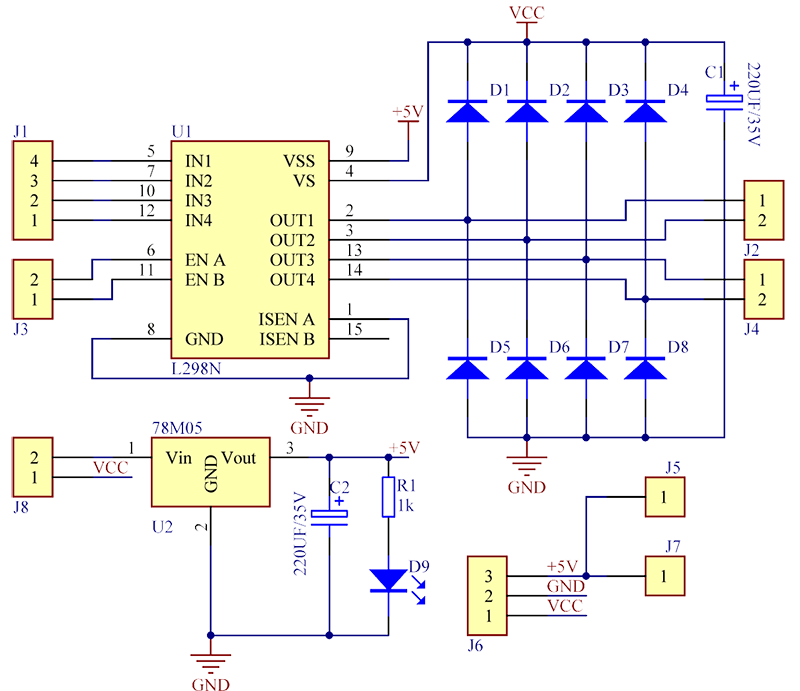
\includegraphics[width=10cm]{images/l298nschematic.png}
        \caption{L298N Schematic}
        \label{fig:l298nschematic}
    \end{center}
\end{figure}

\begin{table}[H]
\centering
\begin{tabular}{ | p{2cm}  p{2cm}  p{2cm} p{3cm}| } 
\hline
\textbf{M0} & \textbf{M1} & \textbf{M2} & \textbf{Resolution} \\
\hline
\hline
Low & Low & Low & Full Step\\
High & Low & Low & Half Step\\
Low & High & Low & 1/4 Step\\
High & High & Low & 1/8 Step\\
Low & Low & High & 1/16 Step\\
High & Low & High & 1/32 Step\\
Low & High & High & 1/32 Step\\
High & High & High & 1/32 Step\\
 \hline
\end{tabular}
\caption{Steps Resolution}
 \label{tab:steps}
 \end{table}
 \begin{figure}[H]
    \begin{center}
        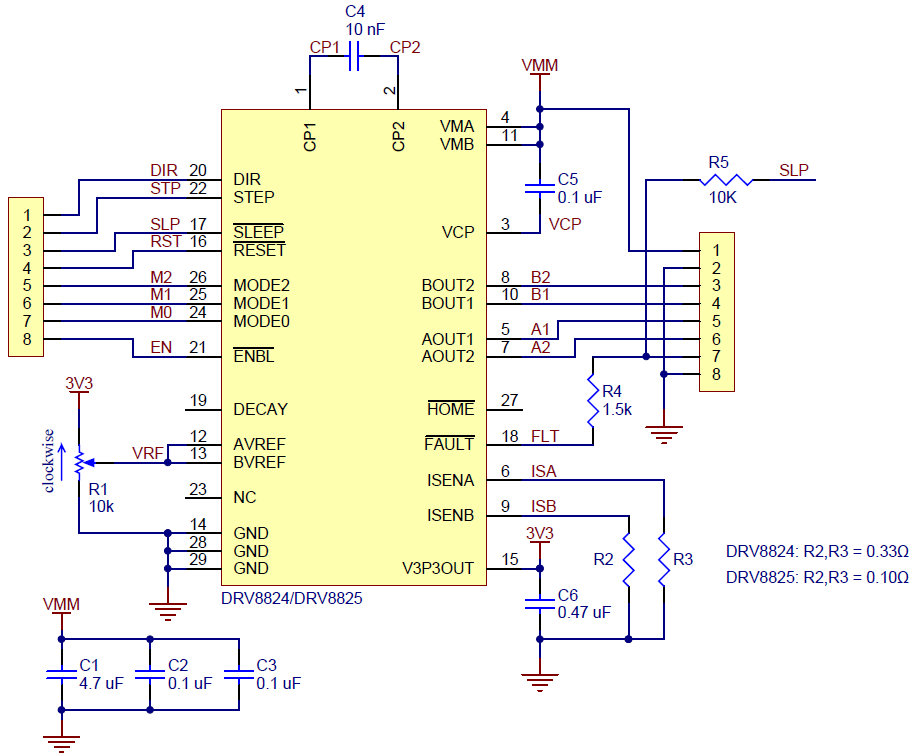
\includegraphics[width=12cm]{images/drv8825schematic.png}
        \caption{DRV8825 Schematic}
        \label{fig:drv8825schematic}
    \end{center}
\end{figure}
 \begin{figure}[H]
    \begin{center}
        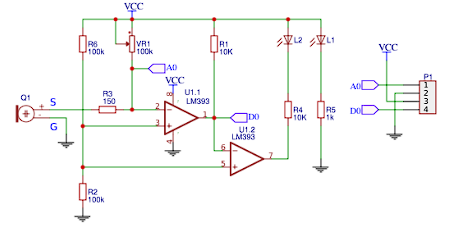
\includegraphics[width=12cm]{images/ky-037schematic.png}
        \caption{ky-037 Schematic}
        \label{fig:ky-037schematic}
    \end{center}
\end{figure}
 \begin{figure}[H]
    \begin{center}
        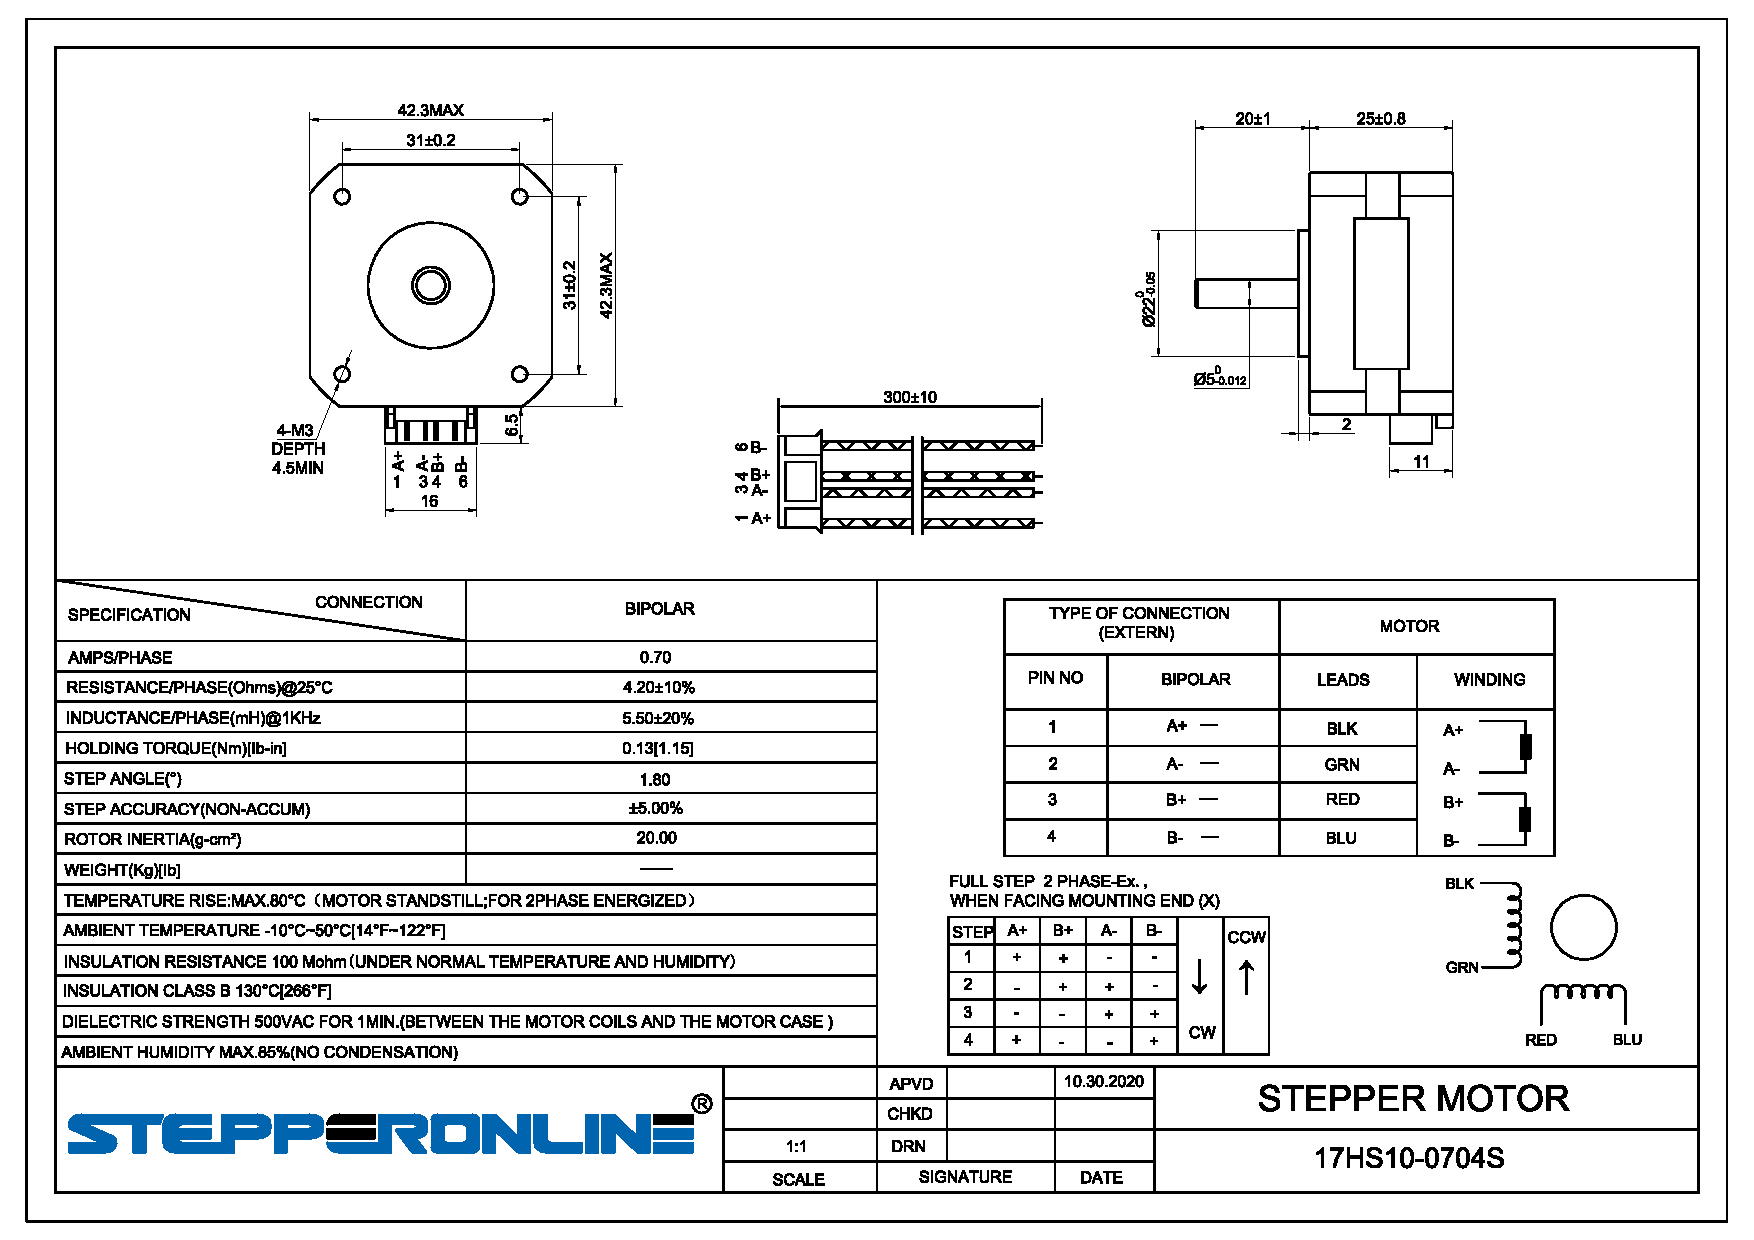
\includegraphics[width=14cm]{images/17HS10-0704S.pdf}
        \caption{NEMA17HS10 from \href{http://www.omc-stepperonline.com}{Stepperonline}}
        \label{fig:NEMA17HS10}
    \end{center}
\end{figure}
\begin{figure}[H]
    \begin{center}
        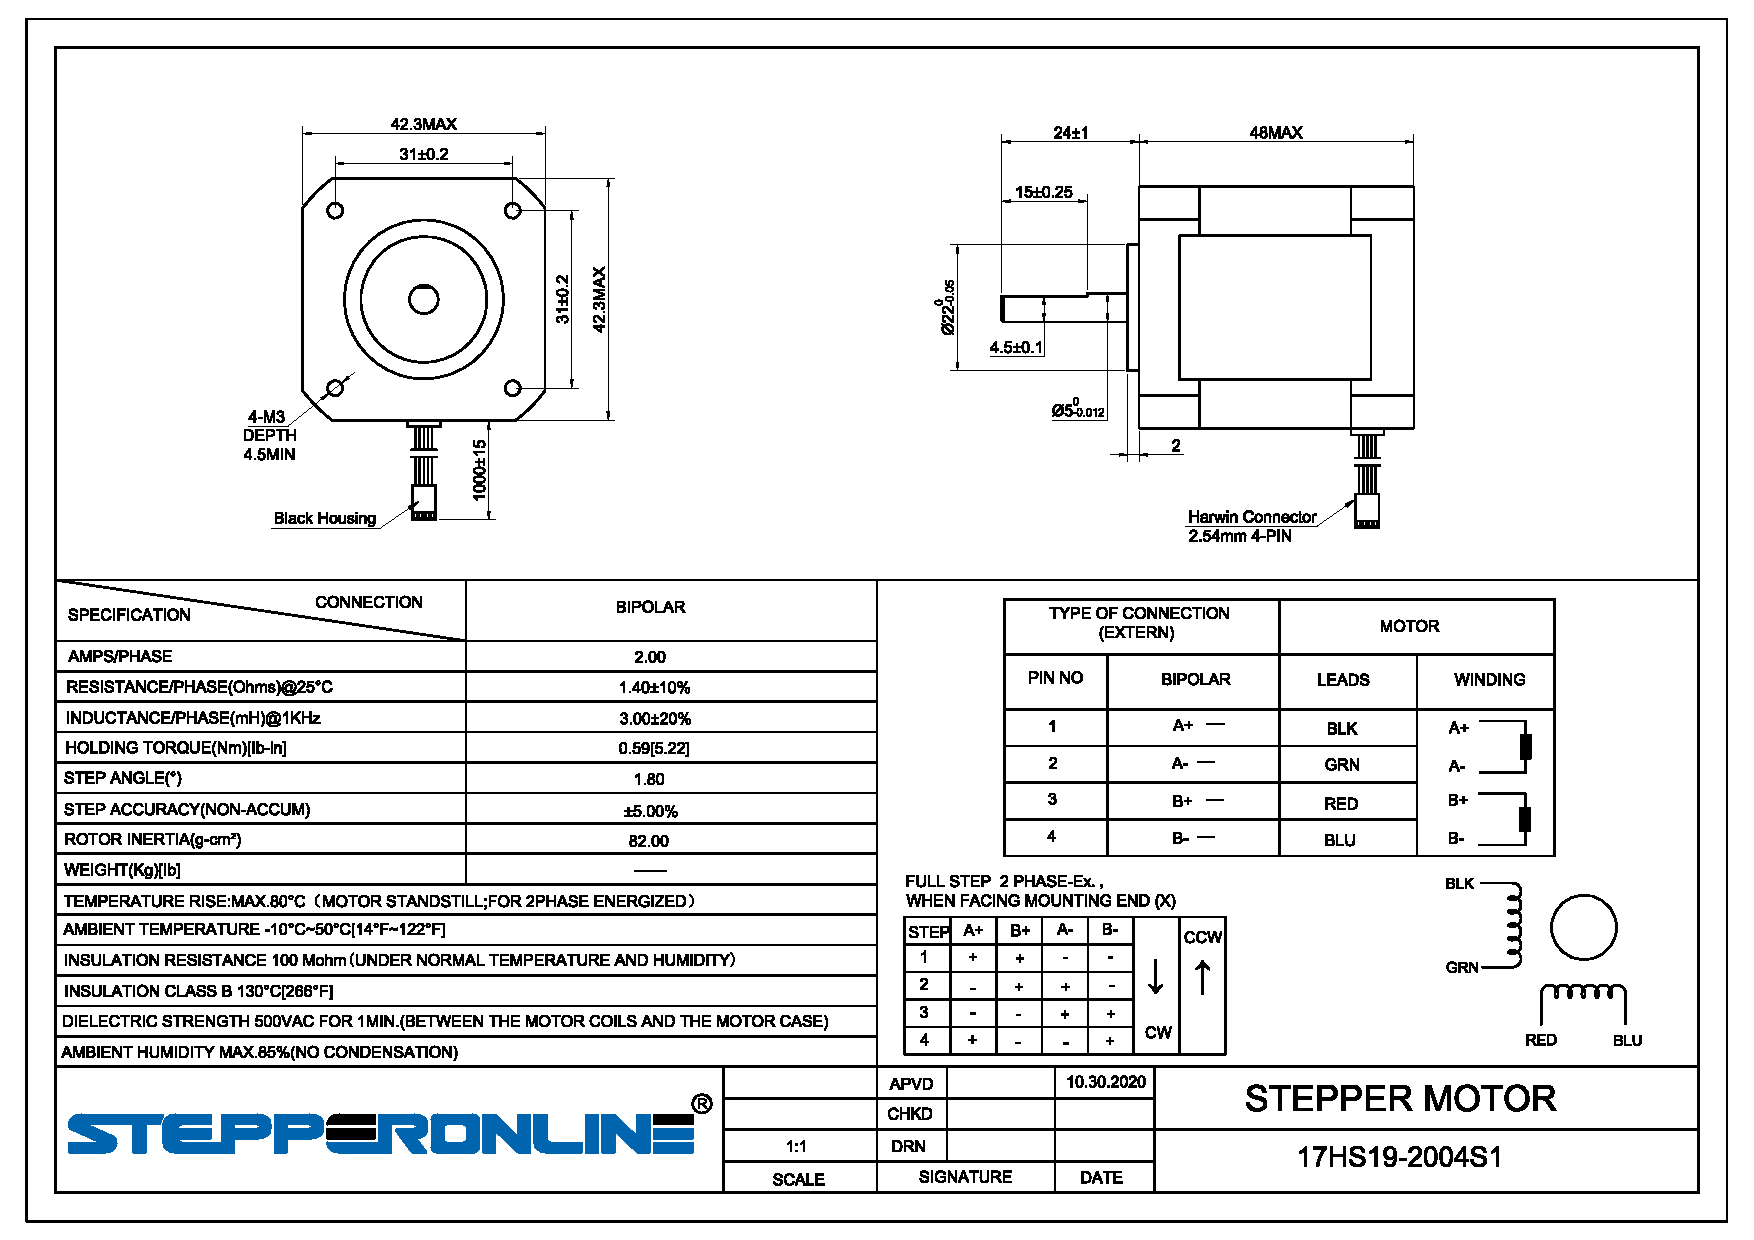
\includegraphics[width=14cm]{images/17HS19-2004S1.pdf}
        \caption{NEMA17HS19 from \href{http://www.omc-stepperonline.com}{Stepperonline}}
        \label{fig:NEMA17HS19}
    \end{center}
\end{figure}
\begin{figure}[H]
    \begin{center}
        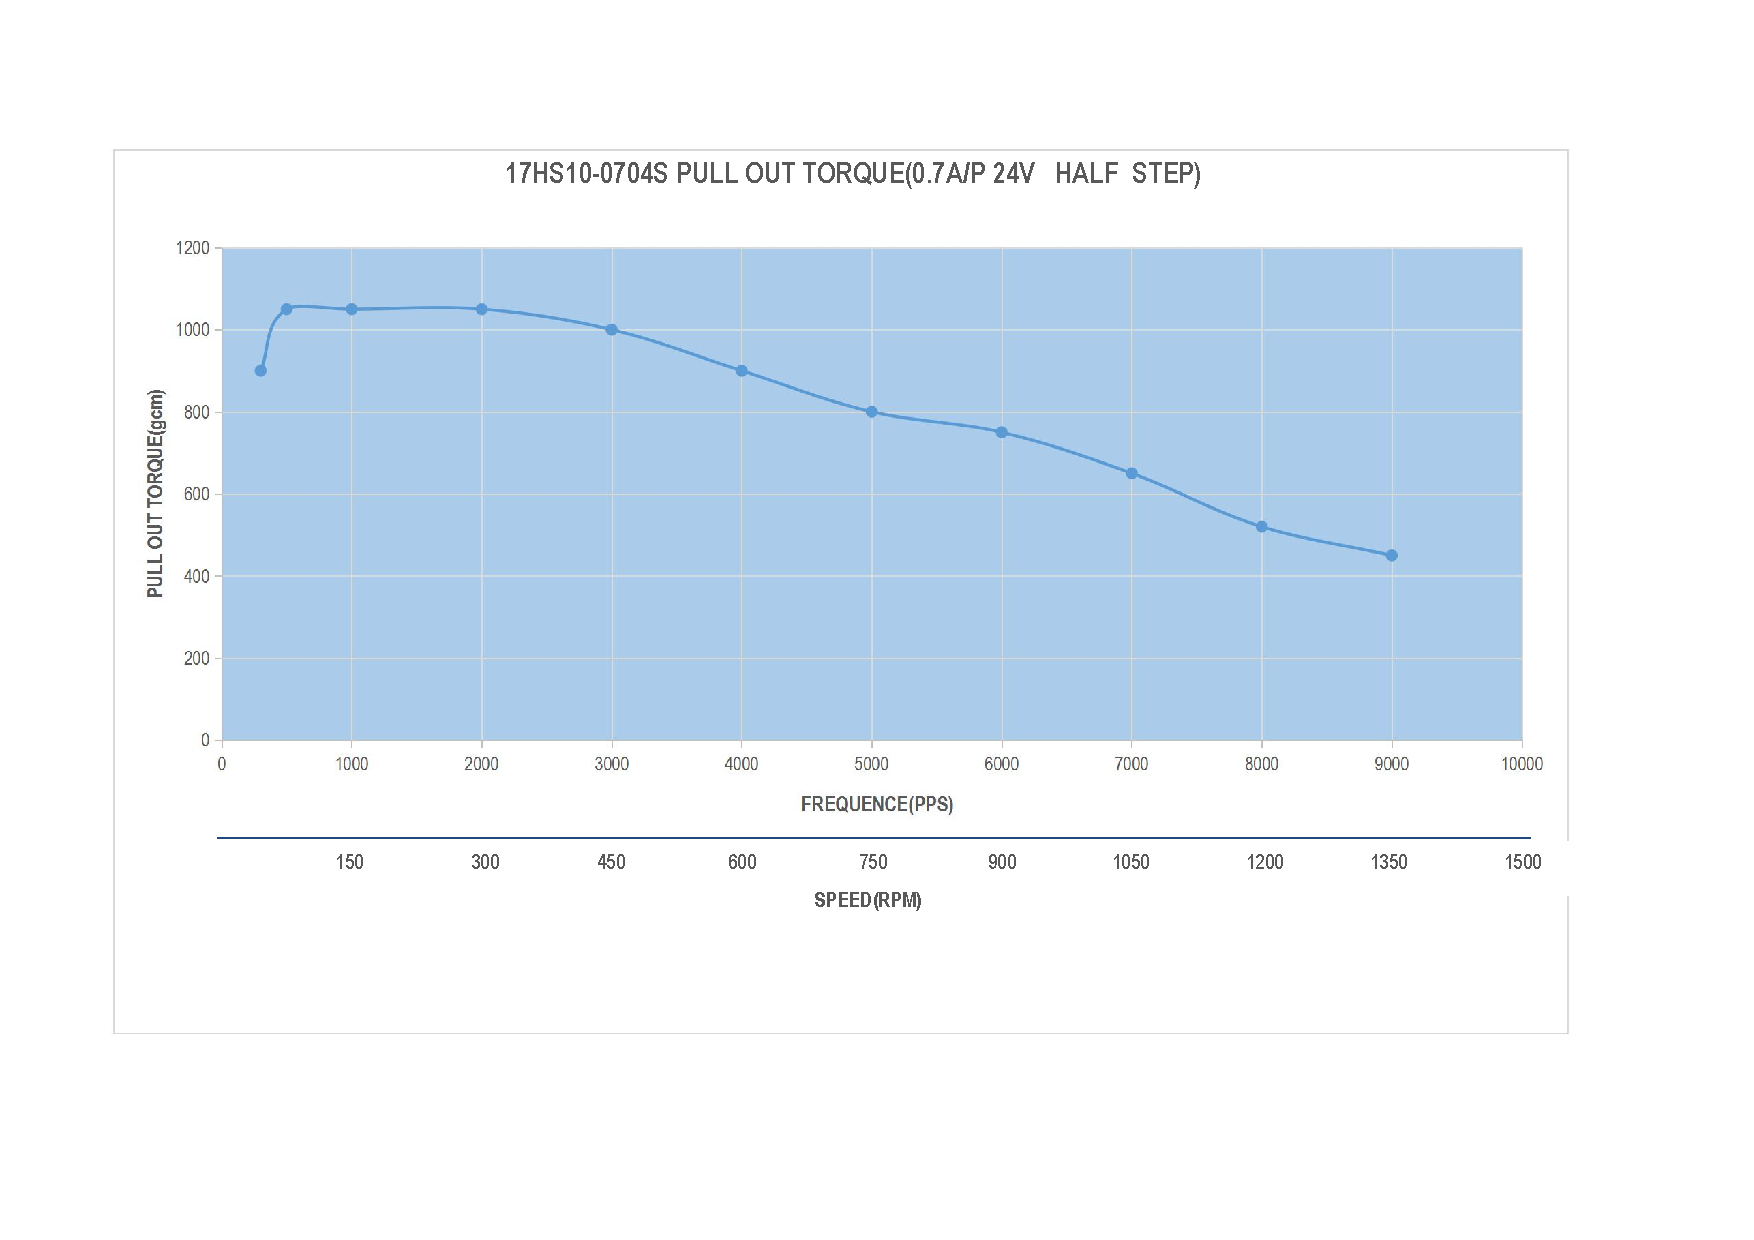
\includegraphics[width=14cm]{images/17HS10-0704S_Torque_Curve.pdf}
        \caption{NEMA17HS10 Torque Curve from \href{http://www.omc-stepperonline.com}{Stepperonline}}
        \label{fig:NEMA17HS10torque}
    \end{center}
\end{figure}
\begin{figure}[H]
    \begin{center}
        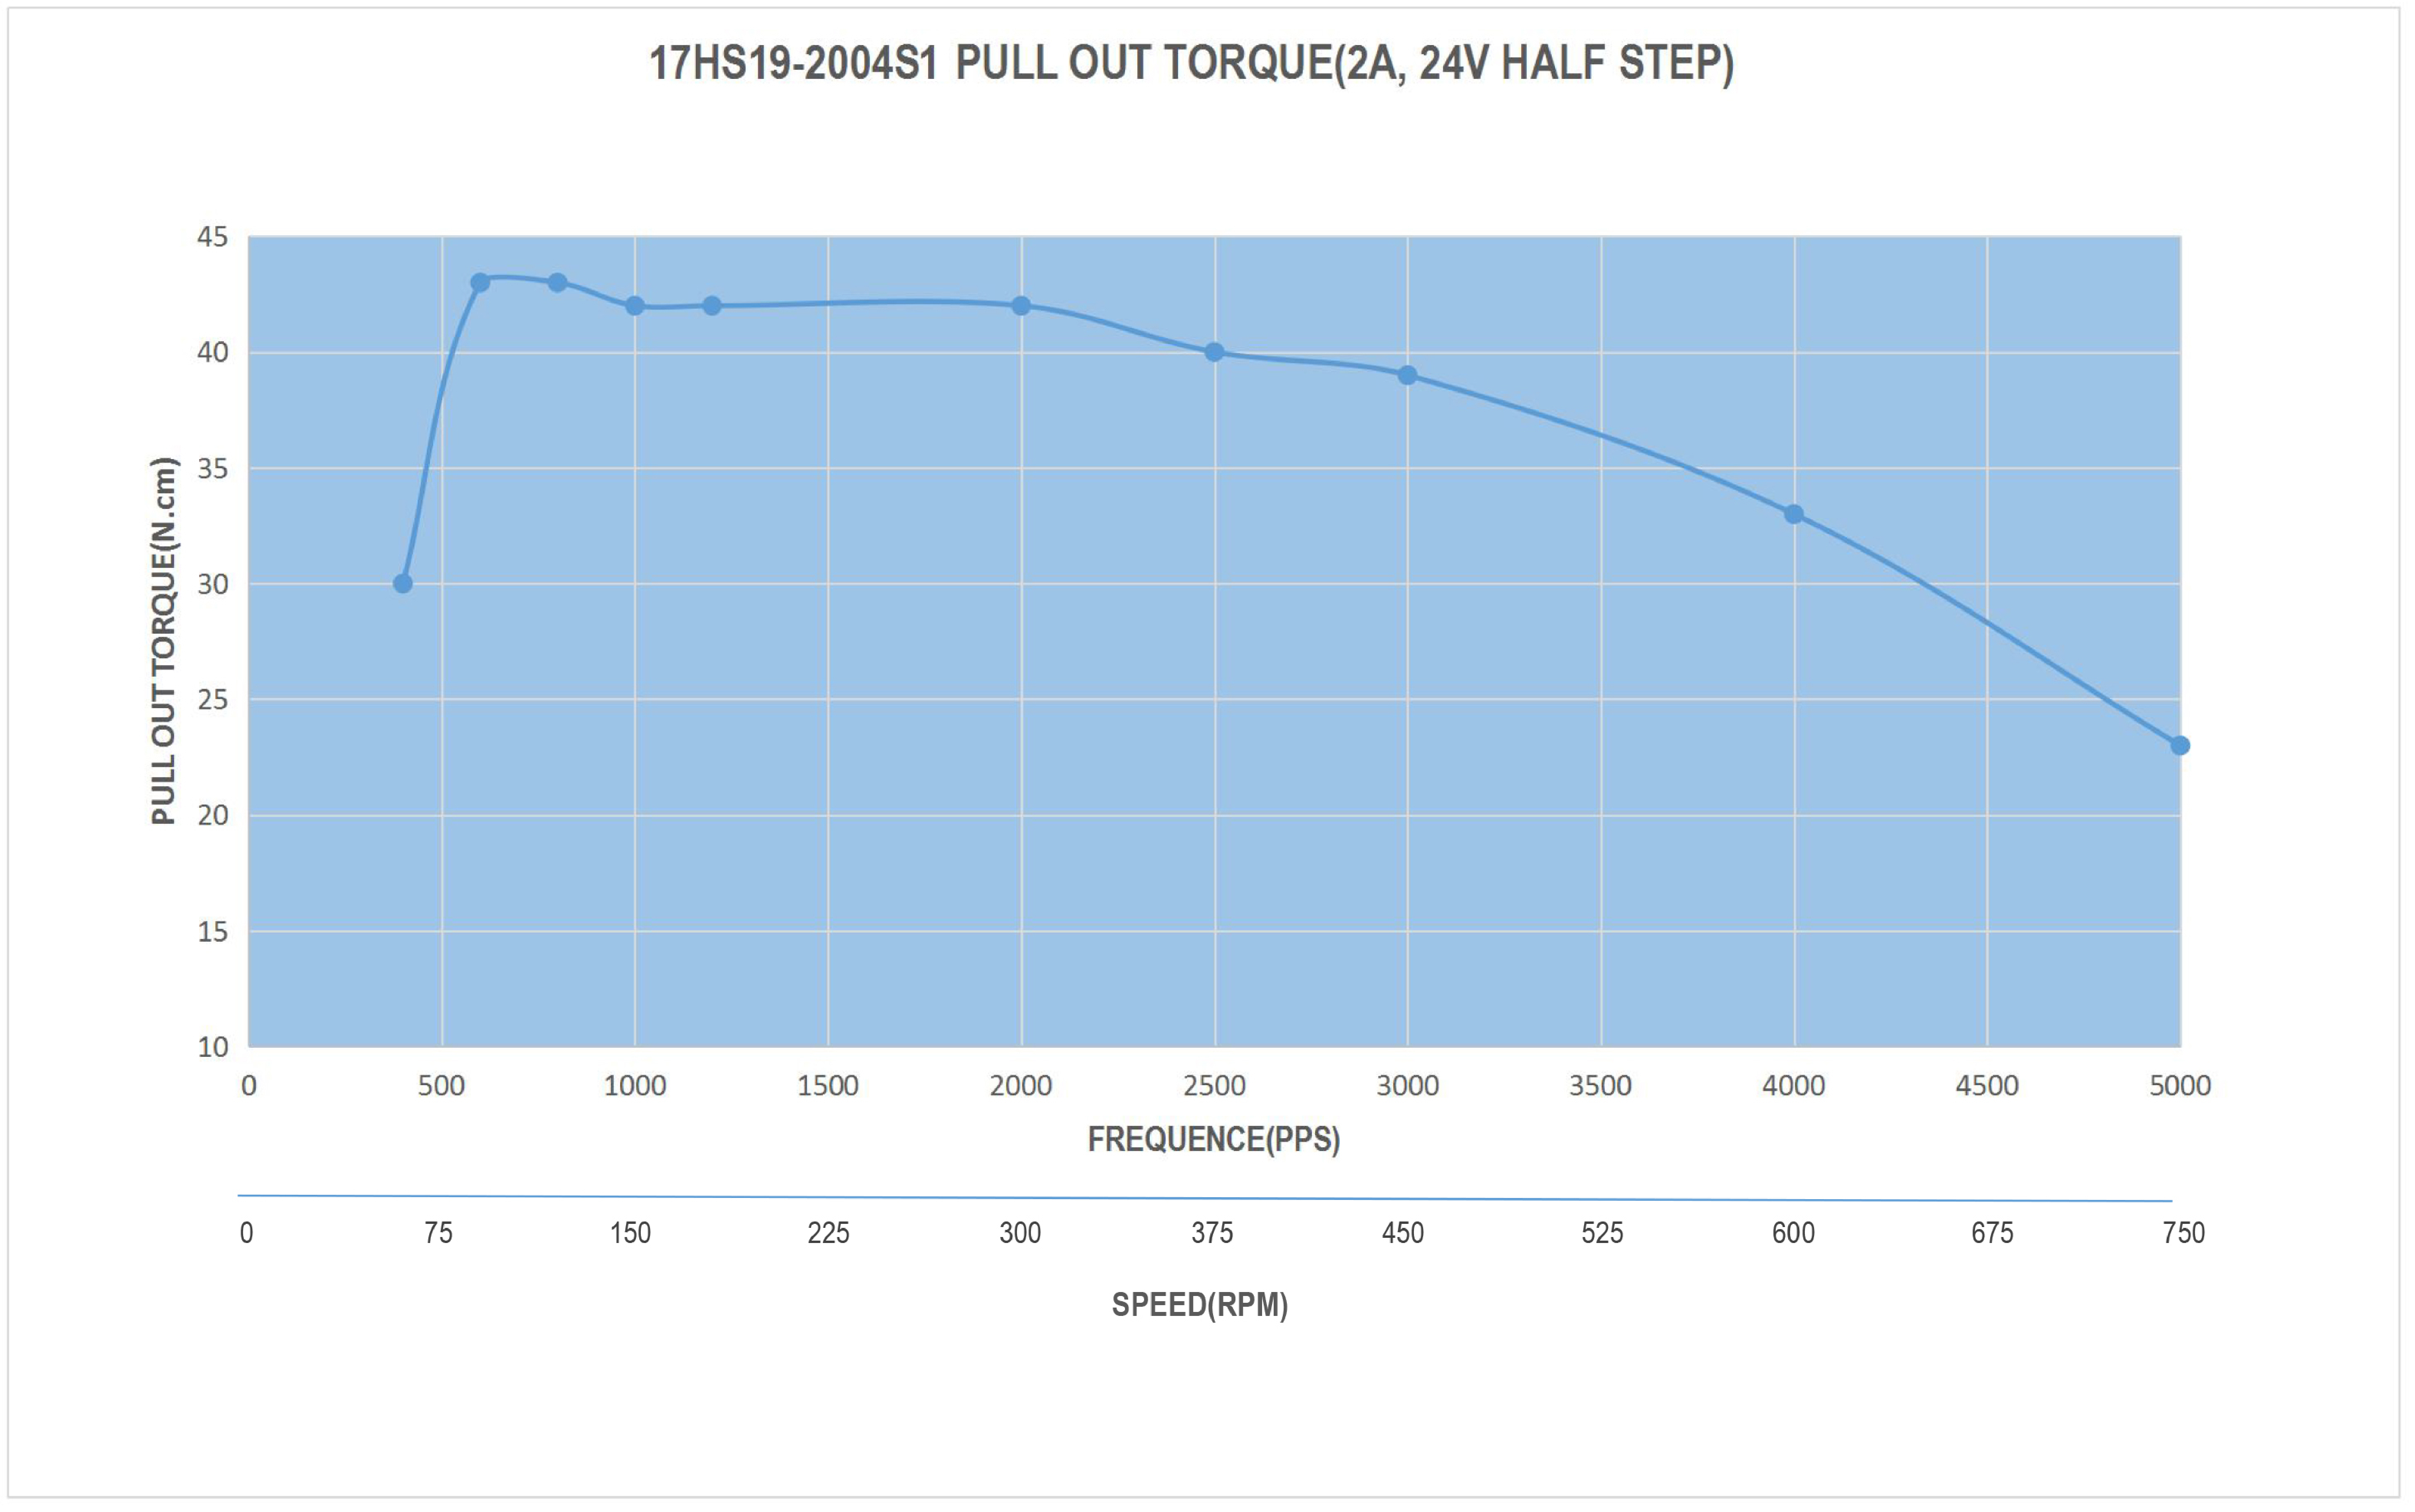
\includegraphics[width=14cm]{images/17HS19-2004S1_Torque_Curve.pdf}
        \caption{NEMA17HS19 Torque Curve from \href{http://www.omc-stepperonline.com}{Stepperonline}}
        \label{fig:NEMA17HS19torque}
    \end{center}
\end{figure}
\begin{figure}[H]
    \begin{center}
        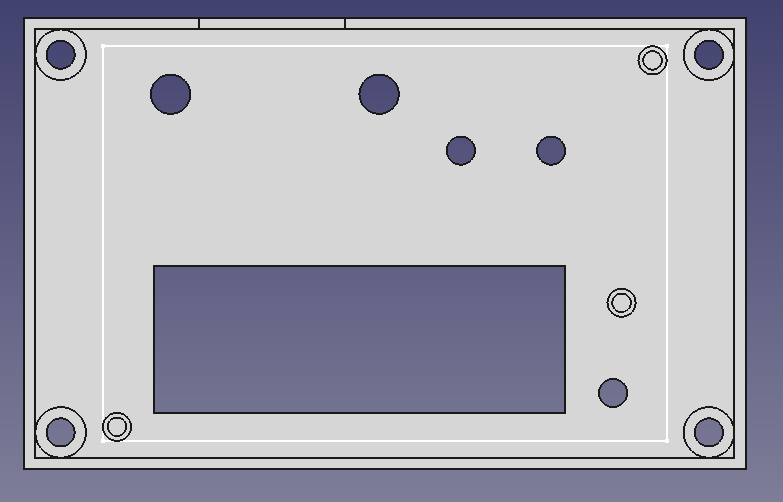
\includegraphics[width=14cm]{images/top_container.PNG}
        \caption{Top section of the Box}
        \label{fig:topbox}
    \end{center}
\end{figure}
\begin{figure}[H]
    \begin{center}
        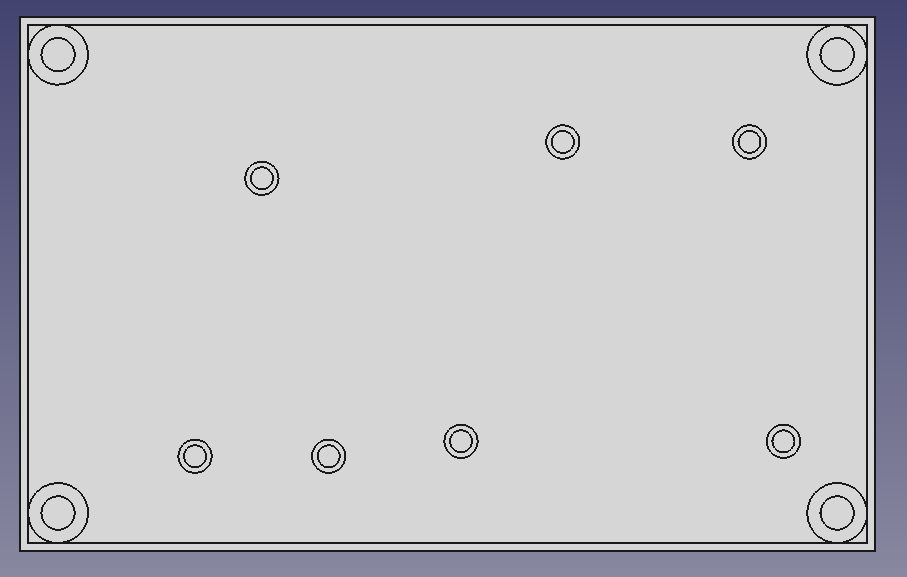
\includegraphics[width=14cm]{images/bottom_container.PNG}
        \caption{Bottom section of the Box}
        \label{fig:botbox}
    \end{center}
\end{figure}
\begin{figure}[H]
    \begin{center}
        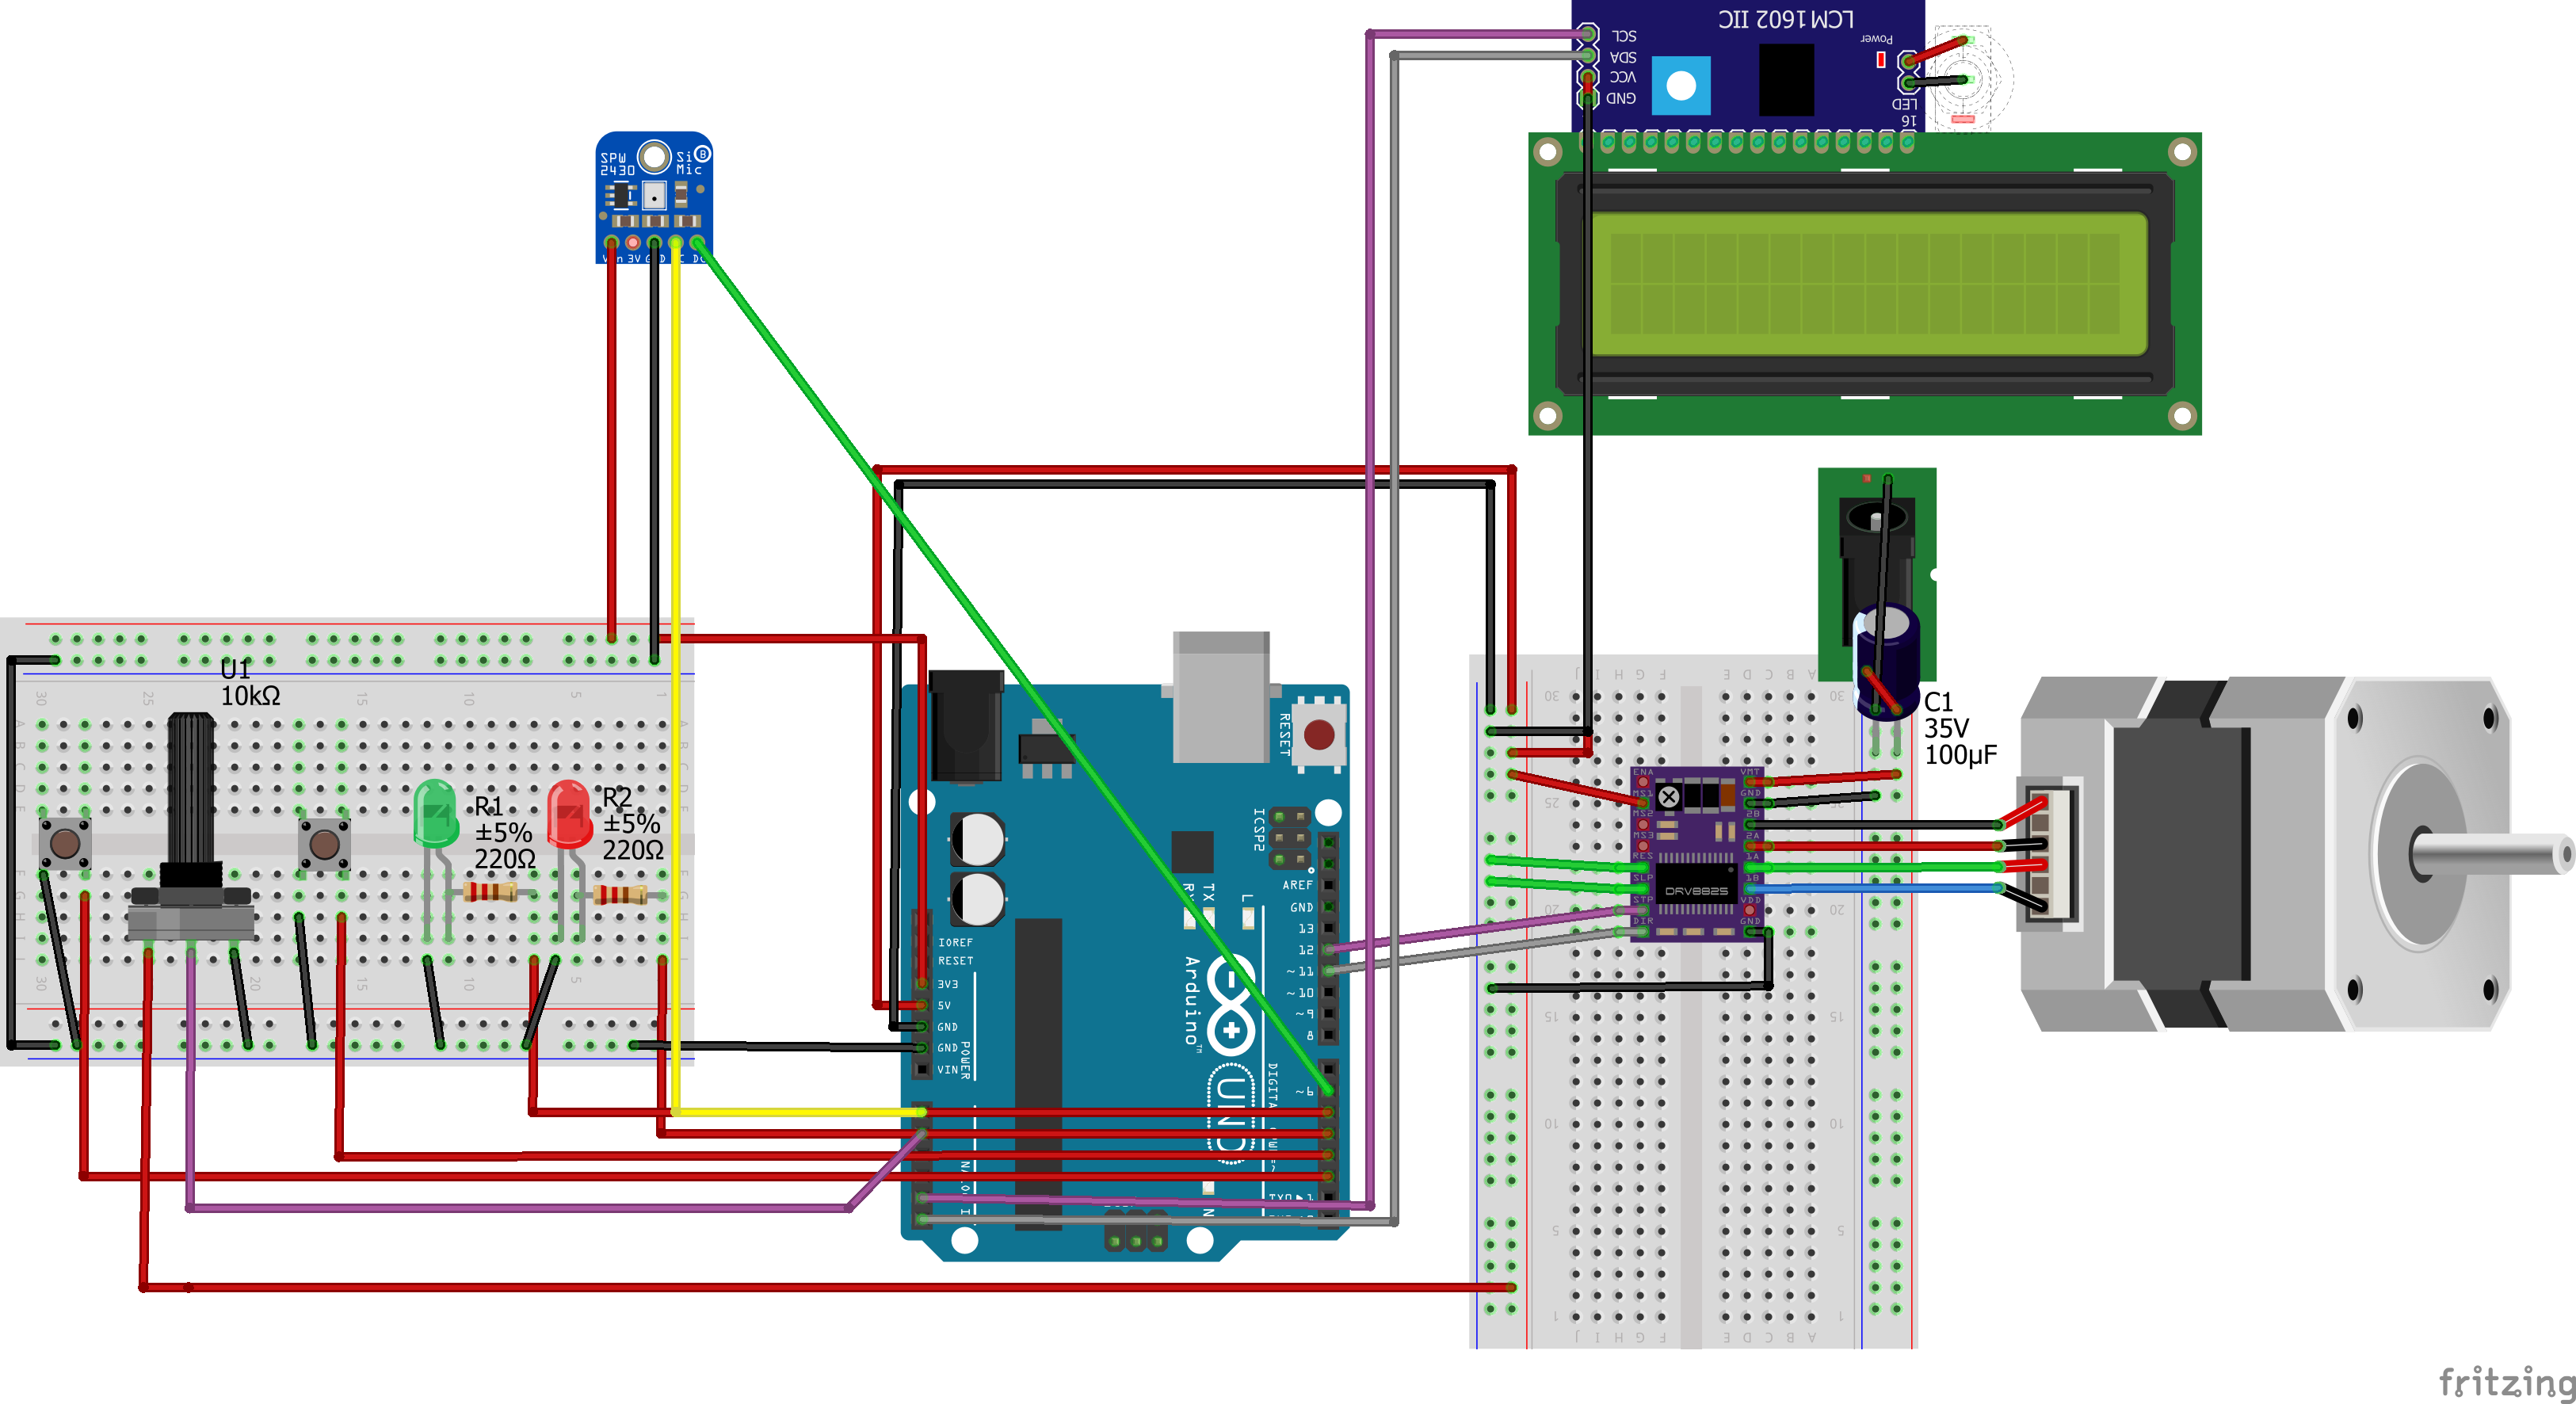
\includegraphics[width=14cm]{images/circuit.PNG}
        \caption{Circuit pinout}
        \label{fig:pinout}
    \end{center}
\end{figure}

\begin{figure}[H]
    \begin{center}
        \includegraphics[width=14cm]{images/final.jpg}
        \caption{Final product}
        \label{fig:final}
    \end{center}
\end{figure}

\end{document}